% Options for packages loaded elsewhere
\PassOptionsToPackage{unicode}{hyperref}
\PassOptionsToPackage{hyphens}{url}
\PassOptionsToPackage{dvipsnames,svgnames,x11names}{xcolor}
%
\documentclass[
  10pt,
  a4paper,
]{scrreprt}

\usepackage{amsmath,amssymb}
\usepackage{iftex}
\ifPDFTeX
  \usepackage[T1]{fontenc}
  \usepackage[utf8]{inputenc}
  \usepackage{textcomp} % provide euro and other symbols
\else % if luatex or xetex
  \usepackage{unicode-math}
  \defaultfontfeatures{Scale=MatchLowercase}
  \defaultfontfeatures[\rmfamily]{Ligatures=TeX,Scale=1}
\fi
\usepackage{lmodern}
\ifPDFTeX\else  
    % xetex/luatex font selection
\fi
% Use upquote if available, for straight quotes in verbatim environments
\IfFileExists{upquote.sty}{\usepackage{upquote}}{}
\IfFileExists{microtype.sty}{% use microtype if available
  \usepackage[]{microtype}
  \UseMicrotypeSet[protrusion]{basicmath} % disable protrusion for tt fonts
}{}
\makeatletter
\@ifundefined{KOMAClassName}{% if non-KOMA class
  \IfFileExists{parskip.sty}{%
    \usepackage{parskip}
  }{% else
    \setlength{\parindent}{0pt}
    \setlength{\parskip}{6pt plus 2pt minus 1pt}}
}{% if KOMA class
  \KOMAoptions{parskip=half}}
\makeatother
\usepackage{xcolor}
\usepackage[inner=2cm,outer=2cm,top=2cm,bottom=2cm,headsep=22pt,headheight=11pt,footskip=33pt,ignorehead,ignorefoot,heightrounded]{geometry}
\setlength{\emergencystretch}{3em} % prevent overfull lines
\setcounter{secnumdepth}{1}
% Make \paragraph and \subparagraph free-standing
\ifx\paragraph\undefined\else
  \let\oldparagraph\paragraph
  \renewcommand{\paragraph}[1]{\oldparagraph{#1}\mbox{}}
\fi
\ifx\subparagraph\undefined\else
  \let\oldsubparagraph\subparagraph
  \renewcommand{\subparagraph}[1]{\oldsubparagraph{#1}\mbox{}}
\fi


\providecommand{\tightlist}{%
  \setlength{\itemsep}{0pt}\setlength{\parskip}{0pt}}\usepackage{longtable,booktabs,array}
\usepackage{calc} % for calculating minipage widths
% Correct order of tables after \paragraph or \subparagraph
\usepackage{etoolbox}
\makeatletter
\patchcmd\longtable{\par}{\if@noskipsec\mbox{}\fi\par}{}{}
\makeatother
% Allow footnotes in longtable head/foot
\IfFileExists{footnotehyper.sty}{\usepackage{footnotehyper}}{\usepackage{footnote}}
\makesavenoteenv{longtable}
\usepackage{graphicx}
\makeatletter
\def\maxwidth{\ifdim\Gin@nat@width>\linewidth\linewidth\else\Gin@nat@width\fi}
\def\maxheight{\ifdim\Gin@nat@height>\textheight\textheight\else\Gin@nat@height\fi}
\makeatother
% Scale images if necessary, so that they will not overflow the page
% margins by default, and it is still possible to overwrite the defaults
% using explicit options in \includegraphics[width, height, ...]{}
\setkeys{Gin}{width=\maxwidth,height=\maxheight,keepaspectratio}
% Set default figure placement to htbp
\makeatletter
\def\fps@figure{htbp}
\makeatother
\newlength{\cslhangindent}
\setlength{\cslhangindent}{1.5em}
\newlength{\csllabelwidth}
\setlength{\csllabelwidth}{3em}
\newlength{\cslentryspacingunit} % times entry-spacing
\setlength{\cslentryspacingunit}{\parskip}
\newenvironment{CSLReferences}[2] % #1 hanging-ident, #2 entry spacing
 {% don't indent paragraphs
  \setlength{\parindent}{0pt}
  % turn on hanging indent if param 1 is 1
  \ifodd #1
  \let\oldpar\par
  \def\par{\hangindent=\cslhangindent\oldpar}
  \fi
  % set entry spacing
  \setlength{\parskip}{#2\cslentryspacingunit}
 }%
 {}
\usepackage{calc}
\newcommand{\CSLBlock}[1]{#1\hfill\break}
\newcommand{\CSLLeftMargin}[1]{\parbox[t]{\csllabelwidth}{#1}}
\newcommand{\CSLRightInline}[1]{\parbox[t]{\linewidth - \csllabelwidth}{#1}\break}
\newcommand{\CSLIndent}[1]{\hspace{\cslhangindent}#1}

\addtokomafont{disposition}{\rmfamily}
\usepackage{ragged2e}
\usepackage{blindtext}\usepackage{amsthm}
\usepackage{amsthm}
\usepackage{hyperref}
\newtheorem{thm}{Theorem}[subsection]
\renewcommand{\thethm}{\arabic{subsection}.\arabic{thm}}

\makeatletter
\makeatother
\makeatletter
\makeatother
\makeatletter
\@ifpackageloaded{caption}{}{\usepackage{caption}}
\AtBeginDocument{%
\ifdefined\contentsname
  \renewcommand*\contentsname{Table of contents}
\else
  \newcommand\contentsname{Table of contents}
\fi
\ifdefined\listfigurename
  \renewcommand*\listfigurename{List of Figures}
\else
  \newcommand\listfigurename{List of Figures}
\fi
\ifdefined\listtablename
  \renewcommand*\listtablename{List of Tables}
\else
  \newcommand\listtablename{List of Tables}
\fi
\ifdefined\figurename
  \renewcommand*\figurename{Figure}
\else
  \newcommand\figurename{Figure}
\fi
\ifdefined\tablename
  \renewcommand*\tablename{Table}
\else
  \newcommand\tablename{Table}
\fi
}
\@ifpackageloaded{float}{}{\usepackage{float}}
\floatstyle{ruled}
\@ifundefined{c@chapter}{\newfloat{codelisting}{h}{lop}}{\newfloat{codelisting}{h}{lop}[chapter]}
\floatname{codelisting}{Listing}
\newcommand*\listoflistings{\listof{codelisting}{List of Listings}}
\usepackage{amsthm}
\theoremstyle{plain}
\newtheorem{theorem}{Theorem}[section]
\theoremstyle{plain}
\newtheorem{conjecture}{Conjecture}[section]
\theoremstyle{definition}
\newtheorem{definition}{Definition}[section]
\theoremstyle{plain}
\newtheorem{corollary}{Corollary}[section]
\theoremstyle{remark}
\AtBeginDocument{\renewcommand*{\proofname}{Proof}}
\newtheorem*{remark}{Remark}
\newtheorem*{solution}{Solution}
\makeatother
\makeatletter
\@ifpackageloaded{caption}{}{\usepackage{caption}}
\@ifpackageloaded{subcaption}{}{\usepackage{subcaption}}
\makeatother
\makeatletter
\@ifpackageloaded{tcolorbox}{}{\usepackage[skins,breakable]{tcolorbox}}
\makeatother
\makeatletter
\@ifundefined{shadecolor}{\definecolor{shadecolor}{rgb}{.97, .97, .97}}
\makeatother
\makeatletter
\makeatother
\makeatletter
\makeatother
\ifLuaTeX
  \usepackage{selnolig}  % disable illegal ligatures
\fi
\IfFileExists{bookmark.sty}{\usepackage{bookmark}}{\usepackage{hyperref}}
\IfFileExists{xurl.sty}{\usepackage{xurl}}{} % add URL line breaks if available
\urlstyle{same} % disable monospaced font for URLs
\hypersetup{
  pdftitle={Annual Progress Review},
  pdfauthor={Thomas William Boughen},
  colorlinks=true,
  linkcolor={blue},
  filecolor={Maroon},
  citecolor={Blue},
  urlcolor={Blue},
  pdfcreator={LaTeX via pandoc}}

\title{Annual Progress Review}
\author{Thomas William Boughen}
\date{May 31, 2024}

\begin{document}
\cleardoublepage
\thispagestyle{empty}
{\centering
\hbox{}\vskip 0cm plus 1fill
{\Huge\bfseries Annual Progress Review \par}
\vspace{12ex}
{\Large\bfseries Thomas William Boughen \par}
\vspace{3ex}
\vskip 0cm plus 2fill
%{\bfseries\large Doctor of Philosophy \par}
\vspace{3ex}
{\bfseries\large May 31, 2024 \par}
\vspace{12ex}
{
\includegraphics[width=0.1\linewidth]{"imgs/University_of_Newcastle_Coat_of_Arms.png"}\par}
%
%
{\bfseries\large Newcastle University \par}
\vspace{3ex}
%
{\bfseries\large School of Mathematics, Statistics and Physics \par}
%
\vspace{12ex}
%{\small Submitted in total fulfilment of the requirements
%of the degree of Doctor of Philosophy \par}
%}
\footnote{An html version of this report can be found at \url{www.twboughen.github.io/phd/APR/report}}
\justifying
\noindent\ifdefined\Shaded\renewenvironment{Shaded}{\begin{tcolorbox}[breakable, interior hidden, enhanced, boxrule=0pt, frame hidden, sharp corners, borderline west={3pt}{0pt}{shadecolor}]}{\end{tcolorbox}}\fi

\renewcommand*\contentsname{Table of contents}
{
\hypersetup{linkcolor=}
\setcounter{tocdepth}{1}
\tableofcontents
}
\hypertarget{sec-int}{%
\chapter{Introduction}\label{sec-int}}

Since the aim is to gain understanding about the behaviour of the degree
distribution of networks at the right tail, it seems natural to look to
using methods from extreme value theory.

\hypertarget{sec-ext}{%
\chapter{Extreme Value Theory}\label{sec-ext}}

This section begins with a review of the theory and methodology for
modelling the extreme values of continuous random variables, before
moving to considerations for modelling the extreme values of discrete
random variables.

\hypertarget{sec-ce}{%
\section{Continuous Extremes}\label{sec-ce}}

Studying the properties of the extreme values of a random variable first
requires determining what exactly is considered to be an extreme value.
In this section extreme values of two kinds are considered, both of
which can be characterised.

The first kind of extreme value considers the distribution of block
maxima. That is, for a set of independent and identically distributed
(iid) random variables \(X_1,\ldots,X_n\) with common cumulative density
function (cdf) \(F\) what is the limiting distribution of
\(M_n = \max\{X_1,\ldots,X_n\}\)?

Clearly, as \(n\rightarrow \infty\), the block maxima \(M_n\) converges
almost surely to the right endpoint of \(F\). However, standardising the
block maxima allows for some characterisation of the limiting
distribution.

\begin{theorem}[Fisher--Tippett--Gnedenko
Theorem]\protect\hypertarget{thm-evt}{}\label{thm-evt}

With \(X_1, \ldots,X_n \overset{\mathrm{iid}}{\sim} F\) and
\(\{ a_n\}_{n\ge0}, \{ b_n\}_{n\ge0}\) such that:

\[\lim_{n\rightarrow\infty}\Pr\left(\displaystyle\frac{1}{a_n}[M_n-b_n]\le x\right) = G(x),\]
for some non-degenerate \(G\).

Then \(F\) is said to be in the (maximum) domain of attraction of \(G\),
denoted \(F\in\mathcal D(G)\) ,and \(G\) is of one of three types:

\begin{itemize}
\tightlist
\item
  Gumbel: \(\Lambda(x) = \exp\{-\exp(-x)\},\quad x \in \mathbb R\)
\item
  Fréchet:
  \(\Phi_\alpha(x) = \exp\{-x^{-\alpha}\},\quad x\ge 0,\alpha>0\)
\item
  Negative-Weibull:
  \(\Psi_\alpha(x) = \exp\{-x^{-a}\},\quad x<0,\alpha>0\)
\end{itemize}

\end{theorem}

Each of these three types defines a domain of attraction.

\begin{definition}[Domains of
Attraction]\protect\hypertarget{def-doa}{}\label{def-doa}

The three domains of attraction that result from Theorem~\ref{thm-evt}
have the following equivalent conditions:

For a distribution with cdf \(F\) and survival function \(\bar F\) that
has right endpoint \(x_F\) given by: \[
x_F = \sup\{x \in \mathbb R \cup\{\infty\}:F(x)<1\}
\] the distribution belongs to each domain of attraction subject to the
conditions below:

\textbf{If there exists a positive function a}

\begin{itemize}
\tightlist
\item
  Type I/Gumbel/\(\mathcal D(\Lambda)\):
\end{itemize}

\[
\lim_{x\uparrow x_F} \displaystyle\frac{\bar F(x+ta(x))}{\bar F(x)} = e^{-t},\quad \forall t\in\mathbb R
\]

\textbf{If} \(x_F=\infty\):

\begin{itemize}
\tightlist
\item
  Type II/Fréchet/\(\mathcal D (\Phi_\alpha)\):
\end{itemize}

\[
\lim_{x\rightarrow\infty} \displaystyle\frac{\bar F(tx)}{\bar F(x)} = x^{-\alpha}, \quad \forall t>0 \quad \text{ for some } \alpha>0
\]

\textbf{If} \(x_F<\infty\):

\begin{itemize}
\tightlist
\item
  Type III/Negative-Weibull/\(\mathcal D(\Psi_\alpha)\):
\end{itemize}

\[
\lim_{h\downarrow 0}\displaystyle\frac{\bar F(x_F-xh)}{\bar F(x_F-h)} = x^\alpha, \quad\alpha>0
\]

\end{definition}

The parameter \(\alpha\) in Definition~\ref{def-doa} and
Theorem~\ref{thm-evt} is called the extreme value index.

Here, distributions in the Gumbel domain are referred to as light
tailed, distributions in the Negative-Weibull domain are referred to as
short tailed, and those in the Fréchet are referred to as heavy
tailed.This terminology for heavy tailed distributions in different ot
some of the literature that defined a heavy tailed distribution as one
that decays slower than exponential. However the terminology used here
is also widely used.

Throughout this report functions will be referred to as regularly
varying or slowly varying, what is meant by this is formally deined
below:

\begin{definition}[Regular
Variation]\protect\hypertarget{def-rv}{}\label{def-rv}

A positive,real valued, measurable function \(f\) is said to be
regularly varying at infinity with index \(\gamma\) if for all \(t>0\):

\[
\lim_{x\rightarrow\infty}\displaystyle\frac{f(tx)}{f(x)} = x^{\gamma}.
\] If \(\gamma =0\), then \(f\) is instead said to be slowly varying at
infinity.

\end{definition}

Note that the condition for a distribution to belong to the Fréchet
domain of attraction is equivalent to saying that the survival function
\(\bar F\) is regularly varying with index \(-\alpha\).

In addition to heavy tailed distributions it is also useful to define
what will be referred to as super heavy tailed distributions. This term
is often just refers to specific distributions such as the log-Cauchy
,log-Gamma,and log-Weibull distributions but Fraga Alves, Haan, and
Neves (2009) provides a more precise definition below:

\begin{definition}[Super Heavy
Tails]\protect\hypertarget{def-sup}{}\label{def-sup}

A distribution is with survival function \(\bar F\) is said to have
super heavy tails if: \[
\lim_{x\rightarrow\infty}\displaystyle\frac{\bar F(tx)}{\bar F (x)} = 1,\qquad \forall t>0
\] That is, a distribution is called super heavy if its survival
function is slowly varying.

\end{definition}

The three main types of extremal distribution (Gumbel, Fréchet and
Negative-Weibull) can be united into one distribution, called the
Generalised Extreme Value (GEV) distribution.

\begin{definition}[Generalised Extreme Value
Distribution]\protect\hypertarget{def-gev}{}\label{def-gev}

Denoted by \(\text{GEV}(\mu,\sigma,\xi)\) the distribution is
characterised by three parameters \(\mu \in \mathbb R\) the location,
\(\sigma\in \mathbb R^+\) the scale, and the shape \(\xi\in \mathbb R\).
It has support on \(\{x\in \mathbb R:1+\xi(x-\mu)/\sigma > 0\}\) and has
cdf given by:

\[
G(x) = \begin{cases}\exp\left\{-\left(1+\displaystyle\frac{\xi(x-\mu)}{\sigma}\right)_+^{-1/\xi}\right\},&\xi\ne0\\
\exp\left\{-\exp\left(-\displaystyle\frac{x-\mu}{\sigma}\right)\right\},&\xi=0.
\end{cases}
\]

\end{definition}

The three types of extremal distribution are obtained from changing the
shape parameter \(\xi\), which corresponds to \(1/\alpha\) in
Theorem~\ref{thm-evt}. This change is generally made so that the largest
\(\xi\) corresponds to heavier tails of the distribution. Specifically,
\(\xi<0\), \(\xi=0\), \(\xi>0\), correspond to the negative Weibull,
Gumbel and the Fréchet domains of attraction respectively.

Another kind of extreme values are the observations above a large
threshold, like the limiting distribution of block maxima, the limiting
distribution of these extreme values can be characterised by the
generalised pareto (GP) distribution.

\begin{definition}[Generalised Pareto
Distribution]\protect\hypertarget{def-gp}{}\label{def-gp}

Consider a random variable \(X\) with the same cdf \(F\) as in
Theorem~\ref{thm-evt}, the Generalised Pareto (GP) distribution can be
obtained by using the GEV distribution and conditional probability such
that for large enough threshold the GP distribution approximately
describes the conditional distribution of threshold exceedances. More
precisely, for sufficiently large threshold \(u\) and the change of
variable to \(Y=X-u\): \[
\Pr(Y\le y | Y>0) = H(y) = \begin{cases}
1-\left(1+\displaystyle\frac{\xi y}{\sigma}\right)^{-1/\xi},&y>0,\xi\ne 0 \\
1-\exp\left(-\displaystyle\frac{y}{\sigma}\right),&y>0,\xi = 0
\end{cases}
\]

\end{definition}

Since this distribution was obtained using a
\(\text{GEV}(\mu,\sigma^*,\xi)\) the shape parameter \(\xi\) is
identical in both distributions and the shape parameter \(\sigma\) is
defined such that \(\sigma = \sigma^* + \xi(u-\mu)\).

It is also possible to derive the result without using the GEV, as shown
in {[}REF{]}.

\hypertarget{sec-disc}{%
\section{Discrete Extremes}\label{sec-disc}}

A lot of Section~\ref{sec-ce} is appropriate only for continuous random
variables and some of the results may not hold in a discrete setting. In
particular, a continuous distribution \(F\) being in certain domain of
attraction may not necessarily imply that a discretisation of \(F\)
remains in that domain of attraction.

\begin{definition}[Discretisation]\protect\hypertarget{def-disc}{}\label{def-disc}

The discretisation of a distribution with cdf \(F\) is given by

\[F^*(n) = F(n) - F(n-1), \quad n   \in \mathbb Z\]

\end{definition}

Shimura (2012) provides conditions for a discretisation of a continuous
distribution to belong to the same domain of attraction. In particular
the following theorem which corresponds to Theorem 1 in Shimura (2012).

\begin{theorem}[Domain of attraction
consistency]\protect\hypertarget{thm-shimura1}{}\label{thm-shimura1}

~

\begin{enumerate}
\def\labelenumi{(\alph{enumi})}
\tightlist
\item
  Every discretisation of distribution in \(\mathcal D(\Phi_\alpha)\)
  remains in \(\mathcal D(\Phi_\alpha)\).
\item
  The discretisation of a distribution remains in
  \(\mathcal D(\Lambda)\) if and only if the original is in
  \(\mathcal D(\Lambda)\cap \mathcal L\).
\end{enumerate}

Where \(\mathcal L\) is the set of long-tailed distributions that have
the property: \[
\lim_{x\rightarrow \infty}\displaystyle\frac{\overline F(x+1)}{\overline F(x)} = 1   
\]

\end{theorem}

In addition Shimura (2012) introduces a quantity useful for determining
the domain of a attraction that a discrete distribution belongs to.

\begin{definition}[Omega
Function]\protect\hypertarget{def-omega}{}\label{def-omega}

For a distribution \(F\) with survival function \(\overline F\) and some
\(n\in\mathbb Z^+\) let:

\[
\Omega(F,n) = \left(\log\displaystyle\frac{\overline F (n+1)}{\overline F (n+2)}\right)^{-1} - \left(\log\displaystyle\frac{\overline F (n)}{\overline F (n+1)}\right)^{-1}
\]

\end{definition}

This quantity plays an important role in Section~\ref{sec-meth} when
determining the domain of attraction to which the degree distribution of
a network generative model belongs. In particular a discrete
distribution is recoverable to the Fréchet domain of attraction
\(\mathcal D(\Phi_\alpha)\) if: \[
\lim_{n\rightarrow\infty}\Omega(F,n) = \alpha^{-1}
\]

Applying ideas from Section~\ref{sec-ce} to modelling discrete random
variables has been approached from many different directions. What
follows is a overview of some of the approaches that have been taken but
will see use in this report.

Hitz, Davis, and Samorodnitsky (2024) note that using the GP
distribution as an approximation in a discrete setting leads to bias in
the likelihood function and can lead to it being inadequate for
modelling. They propose two other peaks over threshold methods that rely
on parametric families of discrete distributions. The first, what they
refer to as the discrete generalised Pareto approximation is based on an
extension of the discrete survival function. The second, the generalised
Zipf distribution is obtained from an extension of the probability mass
function. Both methods are motivated theoretically for modelling of a
large class of discrete distributions and are shown in the paper to
either match or outperform using the GP to model discrete data directly.

Ahmad, Gaetan, and Naveau (2022) first introduce an extended GP
distribution, a continuous distribution that extends the idea of
obtaining GP values from a probability integral transform (PIT) of
\(U(0,1)\) draws and instead considers a PIT of draws from any
distribution on \((0,1)\) such as a beta distribution. This distribution
is then discretised into their discrete extended GP distribution.

The approach that will be used in Section~\ref{sec-meth} follows
{[}ROHRBECK{]}, and first requires defining a discretisation of the GP
distribution.

\begin{definition}[Intergral Generalised Pareto Distribution
(IGP)]\protect\hypertarget{def-igp}{}\label{def-igp}

Consider a random variable \(X\) with cdf \(F\), and consider the random
variable \(Y=\lfloor X \rfloor\). From Definition~\ref{def-gp},
\(X|X>u \sim GP(\sigma, \xi)\) for some sufficiently large
\(u\in \mathbb R^+\) and it can be obtained that the distribution of
\(Y|Y>u\) has distribution defined below:

\[
\Pr(Y=y>Y>u) = \left(1+\displaystyle\frac{\xi(y+1-\lceil u\rceil)}{\sigma_0+\xi\lceil u\rceil}\right)_+^{-1/\xi}-\left(1+\displaystyle\frac{\xi(y-\lceil u\rceil)}{\sigma_0+\xi\lceil u\rceil}\right)_+^{-1/\xi}
\]

For \(y=\lceil u\rceil,\lceil u\rceil+1, \ldots\) and
\(\xi \in \mathbb R\) and \(u, \sigma_0 \in \mathbb R^+.\)

\end{definition}

\hypertarget{sec-mod}{%
\section{Modelling}\label{sec-mod}}

The results from Section~\ref{sec-ce} allow the GEV and GP to be fitted
to the block maxima and exceedances respectively. An example of where
modelling the GEV may be useful are when modelling monthly high
temperatures, fitting the GEV to historic data of peak monthly
temperatures may allow for future prediction of these temperatures.
Fitting the GP may be useful in other scenarios such as modelling the
strength of solar flares.

Typically, when fitting the GP, a sufficiently high threshold needs to
be specified beforehand. {[}COLES{]} provides some empirical methods for
specifying the threshold, one approach is to use a threshold stability
plot that uses maximum likelihood to estimate the parameters of the GP
for a large range of thresholds. The threshold can be chosen as the
point across all of the plots after which the values of the parameters
seems stable. One particular issue when fitting the GP to data, is that
the likelihoods cannot be compared for different thresholds as changing
the threshold changes the amount of data being used.

Another more recent approach shown in {[}MACDONALD 2012{]}, uses a
spliced threshold mixture to model the threshold exceedances where one
distribution is assumed for the bulk of the data and the GP is used for
those values above the threshold. This approach can also be applied in
the discrete setting, and is what is used in Section~\ref{sec-meth}. A
general cases of the model is given below

\begin{definition}[IGP Spliced
Mixture]\protect\hypertarget{def-mixigp}{}\label{def-mixigp}

\[
f(y) = \begin{cases}
(1-\phi)g(x), & y=1,2,\ldots, v\\
\phi\left[\left(1+\displaystyle\frac{\xi(y+1-v)}{\sigma_0+\xi v}\right)_+^{-1/\xi}-\left(1+\displaystyle\frac{\xi(y-v)}{\sigma_0+\xi v}\right)_+^{-1/\xi}\right],&y=v+1, v+2,\ldots
\end{cases}
\] where \(g\) is the pmf of some discrete distribution with support
equal to \(\{1,2,\ldots,v\}\).

\end{definition}

\hypertarget{sec-net}{%
\chapter{Networks}\label{sec-net}}

Networks are the data sources that the results from
Section~\ref{sec-ext} will be used to analyse. Networks appear across a
wide range of fields when attempting to represent complex systems and
the relationships between the components within them.

This section will being with an introduction to the basics of networks
and working with them in mathematics and probability, including the
concept of degree distribution. Then, a look at a few network generation
models and limiting results for the degree distributions of the networks
they generate.

\hypertarget{mathematical-definitions}{%
\section{Mathematical Definitions}\label{mathematical-definitions}}

Throughout this section, graphs constructed from vertices and edges will
be used as an analogue for these networks, so it is appropriate to begin
with some mathematical definitions for exactly what that means.

\begin{definition}[Graph]\protect\hypertarget{def-net}{}\label{def-net}

A graph \(G = (V,E)\) is constructed from a vertex set \(V\) and an edge
set \(E\). The edge set can take on one of two forms depending on if the
graph is directed or un-directed. If the graph is directed then
\(E\subseteq V^2\) i.e the edge set is contained within the set of
ordered pairs of vertices, whereas if the graph is \textbf{un-directed}
then \(E\subseteq [V]^2\), where \[
[V]^2 = \{\{u,v\}:u,v\in V\}
\] i.e.~the edge set is contained within the set of un-ordered pairs of
vertices.

\end{definition}

\begin{definition}[Degree of un-directed
graphs]\protect\hypertarget{def-deg}{}\label{def-deg}

For an un-directed graph a vertex's degree denoted \(d(v)\) for
\(v\in V\) is the number of edges that are connected to vertex \(v\): \[
d(v) = |\{e\in E : v \in e\}|
\]

\end{definition}

\begin{definition}[Degree of directed
graphs]\protect\hypertarget{def-dirdeg}{}\label{def-dirdeg}

Directed graphs have something analogous, called the in-degree
\(d_{in}\), out-degree \(d_{out}\) and total degree \(d_{tot}\). The
in-degree of a vertex \(v\) is the number edges with endpoint at \(v\),
whereas the out-degree is the number of edges with start point at \(v\)
and the total degree is the sum of these i.e.:

\begin{align*}
d_{in}(v)&= |\{(w_1,w_2)\in E: w_2=v \}|\\
d_{out}(v) &= |\{(w_1,w_2)\in E: w_1=v \}|\\
d_{tot}(v) &= d_{in}(v) + d_{out}(v)
\end{align*}

\end{definition}

There are many reasons to analyse network like data, one of which is to
gain an insight into the mechanics that governed the growth of the
network. The next sub-section is focused on presenting several network
generative models, that may be able to describe how real networks grow.
For now, the focus will be on the degree distributions of these network
generative models.

\hypertarget{sec-gen}{%
\section{Network Generative Models}\label{sec-gen}}

It is useful to be able to model the way a network may have grown using
simple rules as the subsequent model can then be used to simulate how
the network may grow in future and provide insights into the underlying
mechanics of the system the network represents. These models are also
sometimes called mechanistic models in the literature. Also, although
they are referred to as network generative models, graphs are still
being used in the rules that govern how the generative model works.

This section begins by detailing a fairly simple generative model and
its limiting results for the degree distribution, followed by two
special cases of the first model and their results.

\hypertarget{general-preferential-attachment-gpa}{%
\subsection{General Preferential Attachment
(GPA)}\label{general-preferential-attachment-gpa}}

Under this model, at each time step one vertex is added to the network
and brings an edge with it that connects the existing vertices with a
probability proportional to some function of the vertices degrees.

\begin{definition}[General Preferential Attachment
Model]\protect\hypertarget{def-gpa}{}\label{def-gpa}

Starting with a graph \(G_1 = (V_1, E_1) = (\{1\}, \emptyset)\), at each
following time step \(t>1\) the graph \(G_t = (V_t, E_t)\) is generated
by the following rules:

\begin{enumerate}
\def\labelenumi{\arabic{enumi}.}
\tightlist
\item
  \textbf{Growth:} Add a new vertex to the vertex set i.e.~\[
  V_t = V_{t-1} \cup \{t\}
  \]
\item
  \textbf{Preferential Attachment:} Add one edge connecting the new
  vertex to one already in the graph \(\{1,\ldots,t-1\}\) selected at
  random with weights proportional to a function of their degree i.e.:
  \[
  E_t  = E_{t-1} \cup \{\tilde e\}
  \] where \(\tilde e_i = \{t,\tilde v\}\) and \(\tilde v = i\) with
  probability \[
  \displaystyle\frac{g(d(i))}{\sum_{w\in V_{t-1}} g(d(i))}, \qquad i\in V_{t-1}
  \]
\end{enumerate}

for some function \(g: \mathbb Z \mapsto \mathbb R^+\setminus\{0\}\),
which will be referred to as the preferential attachment function

\end{definition}

\hypertarget{limiting-degree-distribution}{%
\subsubsection{Limiting Degree
Distribution}\label{limiting-degree-distribution}}

In {[}GPA REF{]} the limiting degree distribution was calculated in
terms of the preferential attachment function and does not have a
general explicit form. It is defined as follows, let \(\lambda^*\) be
the solution, if it exists, to:

\[
1=\sum_{n=1}^\infty \prod_{i=1}^{n-1}\displaystyle\frac{g(i)}{g(i)+\lambda}
\] then the limiting degree distribution of a network resulting from the
GPA model has probability mass function (pmf):

\[
f(k) = \displaystyle\frac{\lambda^*}{g(k) + \lambda^*}\prod_{i=0}^{k-1}\displaystyle\frac{g(i)}{g(i)+\lambda^*}
\]

\hypertarget{barabuxe1si-albert-ba}{%
\subsection{Barabási-Albert (BA)}\label{barabuxe1si-albert-ba}}

The GPA model has several special cases, when \(g\) is the identity
function i.e \(g(k)=k\), it becomes the BA model (Barabási and Albert
1999) with \(m=1\).

\begin{definition}[Barabási-Albert
Model]\protect\hypertarget{def-ba}{}\label{def-ba}

Starting with a graph \(G_1 = (V_1, E_1)\) where
\(V_1 = \{1,\ldots,m_0\}\) and \(E_1 = \{\{v\}:v\in V_1\}\) i.e a graph
with \(m_0\) vertices with one self-loop each. At each time step \(t>1\)
the graph \(G_t = (V_1, E_1)\) is generated by the following rules:

\begin{enumerate}
\def\labelenumi{\arabic{enumi}.}
\tightlist
\item
  \textbf{Growth:} Add a new vertex to the vertex set i.e.~\[
  V_t = V_{t-1} \cup \{t\}
  \]
\item
  \textbf{Preferential Attachment:} Add \(m\le m_0\) edges between the
  new vertex and those already in the graph with probability
  proportional to each vertices degree i.e.~\[
  E_t  = E_{t-1} \cup \{\tilde e_1, \ldots, \tilde e_m\}
  \] where each new edge
  \(\tilde e_i = \{t, \tilde v_i\}\)(\(i=1,\ldots, m\)) has
  \(\tilde v_i\) sampled independently without replacement from
  \(V_{t-1}\) with probability: \[
  \frac{d(\tilde v_i)}{\sum_{u\in V_{t-1}}d(u)}
  \]
\end{enumerate}

\end{definition}

\hypertarget{limiting-degree-distriubtion}{%
\subsubsection{Limiting Degree
Distriubtion}\label{limiting-degree-distriubtion}}

In {[}NETWORK SCI book{]}, it was shown that for large values of \(t\),
the limiting degree distribution of a network produces by this model is:

\[
f(k) = \frac{2m(m+1)}{k(k+1)(k+2)}, \qquad k\geq m
\] According to {[}REF{]} this pmf is regularly varying with exponent 2,
meaning that it is in the Fréchet domain of attraction
\(\mathcal D(\Phi_2)\).

\hypertarget{uniform-attachment-ua}{%
\subsection{Uniform Attachment (UA)}\label{uniform-attachment-ua}}

The final special case presented here is obtained from setting the
preferential attachment function \(g\) to be some constant value.

\begin{definition}[Uniform Attachment
Model]\protect\hypertarget{def-ua}{}\label{def-ua}

Start with a graph \(G_1 = (V_1, E_1) = (\{1,\ldots,m_0\}, \emptyset)\),
at each time step \(t>1\) the graph is denoted by \(G_t=(V_t, E_t)\) and
generated by repeating the following two steps:

\begin{enumerate}
\def\labelenumi{\arabic{enumi}.}
\tightlist
\item
  \textbf{Growth:} Add a new vertex to the vertex set i.e.~\[
  V_t=V_{t-1}\cup\{t\}
  \]
\item
  \textbf{Uniform Attachment:} Add \(m\le m_0\) edges between the new
  vertex and those already in the graph with probability proportional to
  each vertices degree i.e.~\[
  E_t  = E_{t-1} \cup \{\tilde e_1, \ldots, \tilde e_m\}
  \] where each new edge
  \(\tilde e_i = \{t, \tilde v_i\}\)(\(i=1,\ldots, m\)) has
  \(\tilde v_i\) sampled independently without replacement from
  \(V_{t-1}\) with probability: \[
  \frac{1}{\sum_{u\in V_{t-1}}1} = \frac{1}{|V_{t-1}|}
  \]
\end{enumerate}

\end{definition}

\hypertarget{limiting-degree-distribution-1}{%
\subsubsection{Limiting Degree
Distribution}\label{limiting-degree-distribution-1}}

As showing in {[}REF{]} the expected degree distribution of this model
for large values of \(t\) is approximately: \[
f(k) = \displaystyle\frac{e}{m}\exp\left(-\displaystyle\frac{k}{m}\right),\qquad k \ge m
\] Although this was not shown rigourously and treats the degree of a
vertex as a continuous random variable, this is an shifted exponential
distribution with left endpoint \(m\) and rate parameter \(1/m\) and as
such is in the Gumbel domain of attraction.

If \(m=1\), it is possible to get a more precise result from the result
regarding the limiting degree distribution of the GPA. By setting the
preferential attachment function \(g(k) = \lambda^*\), the can be shown
that the limiting degree distribution is: \[
f(k) = \left(\frac{1}{2} \right)^{k}, \qquad k=1,2,\ldots 
\] This distribution also occupies the Gumbel domain of attraction.

\hypertarget{sec-meth}{%
\chapter{Methods}\label{sec-meth}}

The aim of this section is to investigate the degree distribution of
real networks and compare them to the results obtained for the
generative models in Section~\ref{sec-gen}. First, a look at what the
degree distributions of real networks look like.

\begin{figure}[H]

{\centering 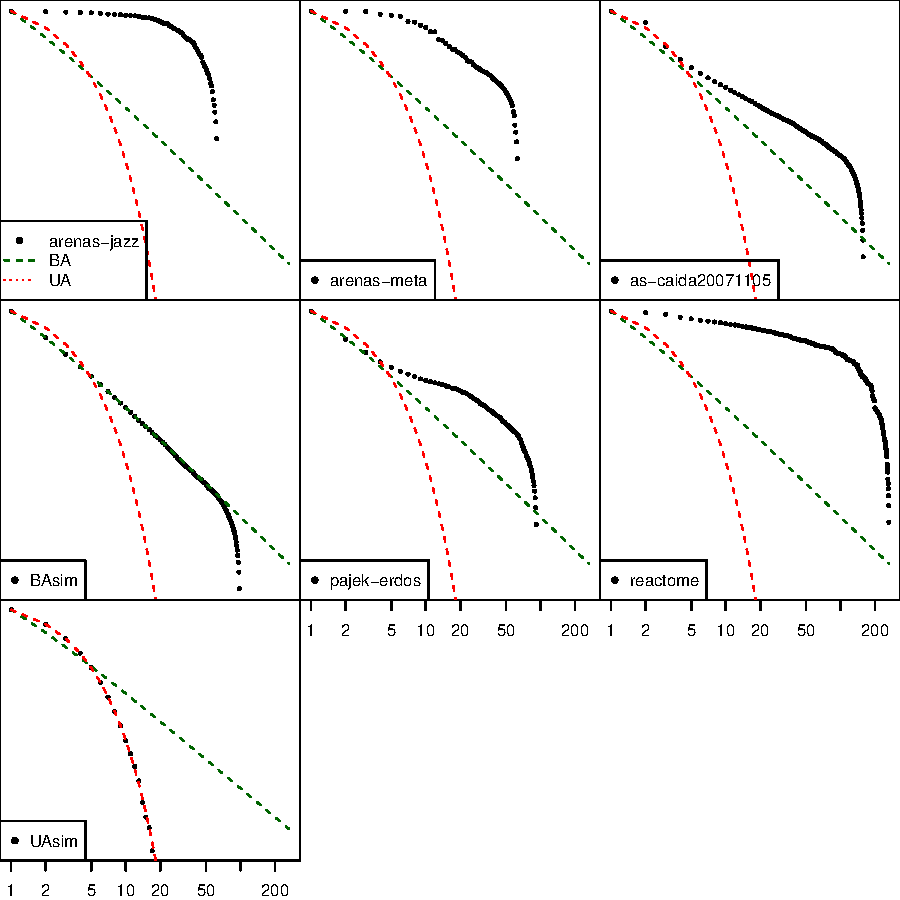
\includegraphics[width=0.66\textwidth,height=\textheight]{doc_files/figure-pdf/fig-survs-1.pdf}

}

\caption{\label{fig-survs}Plots of survial functions of real networks
degrees}

\end{figure}

Figure~\ref{fig-survs} shows the survival function of the degrees of
various real networks as well as ``BAsim'' and ``UAsim'' which were
generated using the corresponding schemes in Section~\ref{sec-gen}.
Additionally, the theoretical limiting degree distribution of both the
UA model and the BA model (for m=1) are included on the plots. Visually
it seems that neither of these models are adequate for modelling the
growth of the real networks shown here.

To further investigate this, Section~\ref{sec-realmodel} considers
fitting a model to these data that will provide insight into what would
be needed from a network generative model such that it flexible enough
to capture the variation of shapes of degree distribution in real
networks.

\hypertarget{sec-realmodel}{%
\section{Modelling degree distributions}\label{sec-realmodel}}

As mentioned in Section~\ref{sec-mod}, the method used here to model the
extreme values of the data will be a spliced threshold mixture.
Specifically, it will be a spliced threshold mixture of a power law and
a discretisation of the generalised pareto distribution similar to what
is defined in {[}ROHRBECK{]}.

\begin{definition}[Power-Law IGP
Distribution]\protect\hypertarget{def-pligp}{}\label{def-pligp}

\[
f(y) = \begin{cases}
(1-\phi)\displaystyle\frac{y^{-(\alpha+1})}{\sum_{k=1}^v}k^{\alpha+1}, & y=1,2,\ldots, v\\
\phi\left[\left(1+\displaystyle\frac{\xi(y+1-v)}{\sigma_0+\xi v}\right)_+^{-1/\xi}-\left(1+\displaystyle\frac{\xi(y-v)}{\sigma_0+\xi v}\right)_+^{-1/\xi}\right],&y=v+1, v+2,\ldots
\end{cases}
\]

\end{definition}

\hypertarget{fitting-model-to-the-data}{%
\section{Fitting model to the data}\label{fitting-model-to-the-data}}

The values of the parameters in the model for each data set were
estimated under the Bayesian framework using a Metropolis within Gibbs
sampler. Below are plots showing the same data as in
Figure~\ref{fig-survs} but with the mean and 95\% confidence intervals
of the survival function of the model for each data-set.

\begin{figure}[H]

{\centering 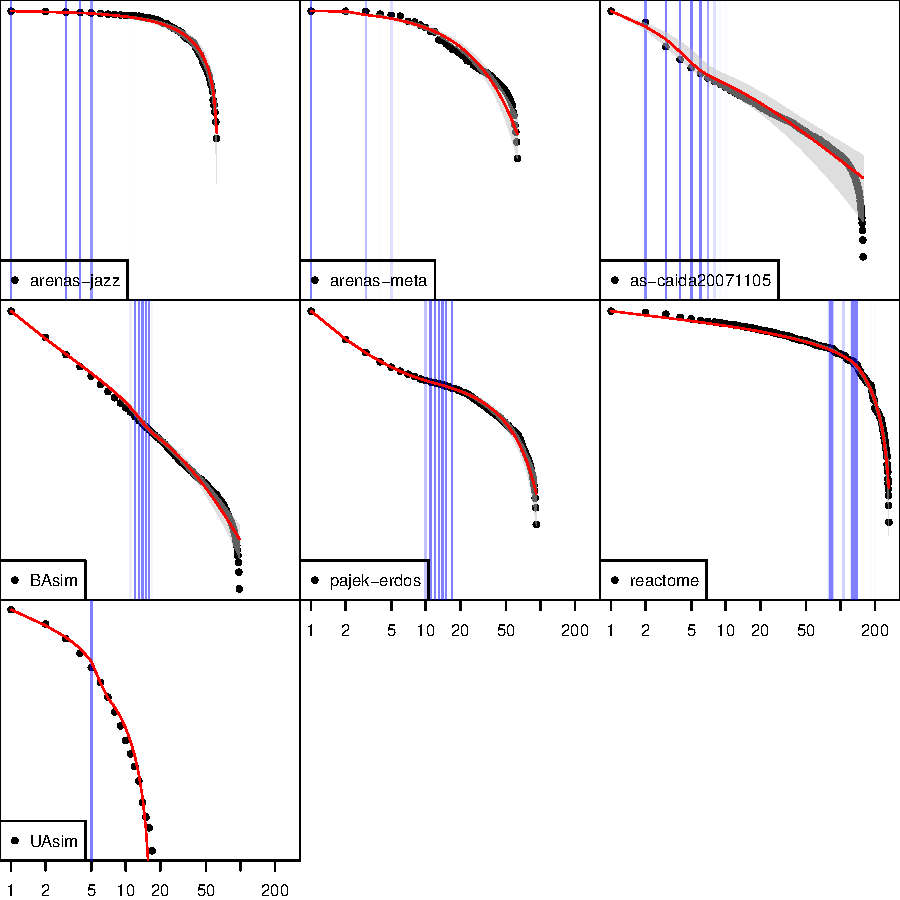
\includegraphics[width=0.66\textwidth,height=\textheight]{doc_files/figure-pdf/fig-fits1-1.pdf}

}

\caption{\label{fig-fits1}Plots of truncated survial functions of real
networks degrees}

\end{figure}

As show by Figure~\ref{fig-fits1} the model seems to fit the data quite
well, below are some plot summarising each of the paramters for each of
the models:

\begin{figure}[H]

{\centering 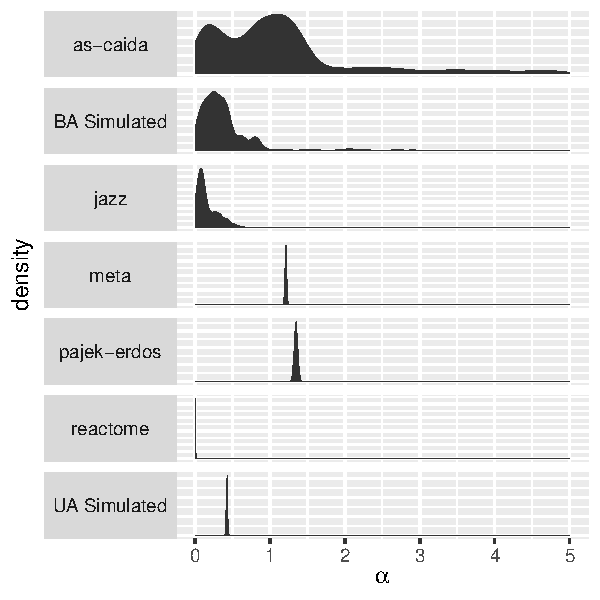
\includegraphics[width=0.75\textwidth,height=\textheight]{doc_files/figure-pdf/fig-alpha-1.pdf}

}

\caption{\label{fig-alpha}Posterior of power law index (\(\alpha\))}

\end{figure}

\begin{figure}[H]

{\centering 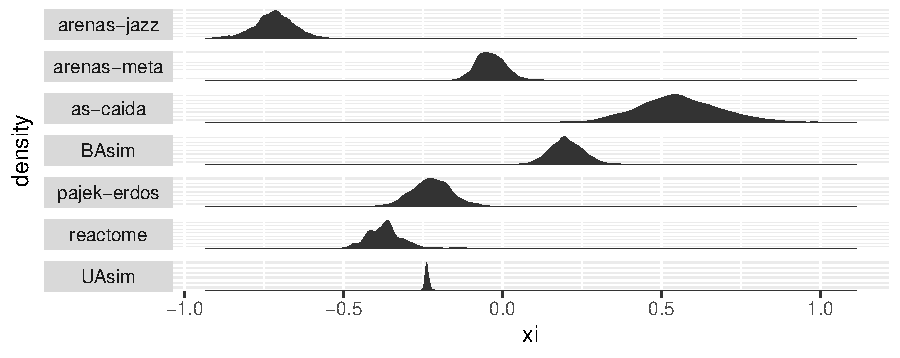
\includegraphics[width=0.75\textwidth,height=\textheight]{doc_files/figure-pdf/fig-shape-1.pdf}

}

\caption{\label{fig-shape}Posterior of shape (\(\xi\))}

\end{figure}

\begin{figure}[H]

{\centering 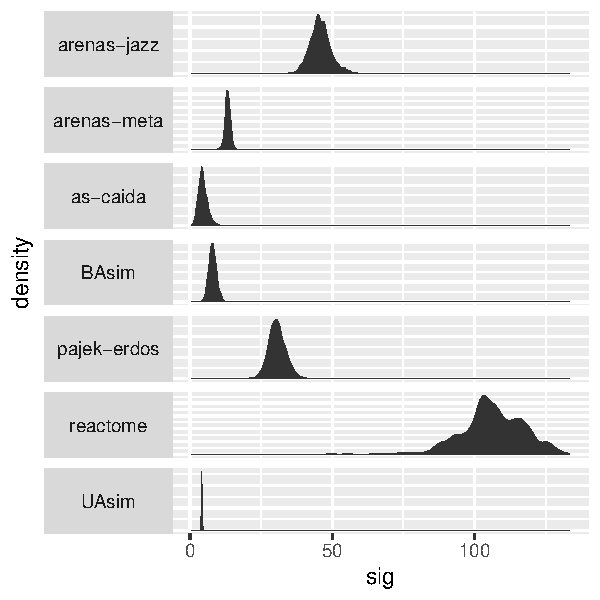
\includegraphics[width=0.75\textwidth,height=\textheight]{doc_files/figure-pdf/fig-scale-1.pdf}

}

\caption{\label{fig-scale}Posterior of scale (\(\sigma\))}

\end{figure}

\begin{figure}[H]

{\centering 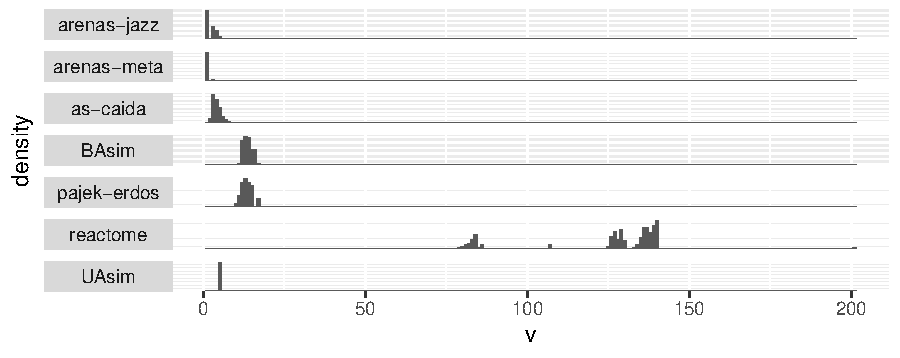
\includegraphics[width=0.75\textwidth,height=\textheight]{doc_files/figure-pdf/fig-thresh-1.pdf}

}

\caption{\label{fig-thresh}Posterior of threshold (\(v\))}

\end{figure}

\hypertarget{gpa-analyses}{%
\section{GPA analyses}\label{gpa-analyses}}

So far it has been shown that neither the BA model nor the UA model can
adequately capture the range of type of degree distributions of real
networks. So, a natural place to start when attempting to expand the
range of possible degree distributions is the more general model, the
GPA. This section, will use results from Shimura (2012) and
Section~\ref{sec-ext} to investigate the possible types of degree
distribution that may arise from different preferential attachment
functions in the GPA model.

\hypertarget{the-preferential-attachment-function}{%
\subsection{The Preferential Attachment
Function}\label{the-preferential-attachment-function}}

From here on the preferential functions that will be used for the GPA
model will be of the form: \[
g(k) = k^\gamma, \qquad \gamma>0.
\]

This allows for investigating the cases where the preferential
attachment function is sub-linear and when it is super-linear.

\hypertarget{section}{%
\subsection{}\label{section}}

As discussed in Section~\ref{sec-disc}, the limiting value of
\(\Omega(F,n)\) can give a lot of information about the behaviour of a
discrete distribution at extreme values. Below is a plot showing the
value of this quantity as \(n\) increases for various different values
of \(\gamma\).

\begin{figure}[H]

{\centering 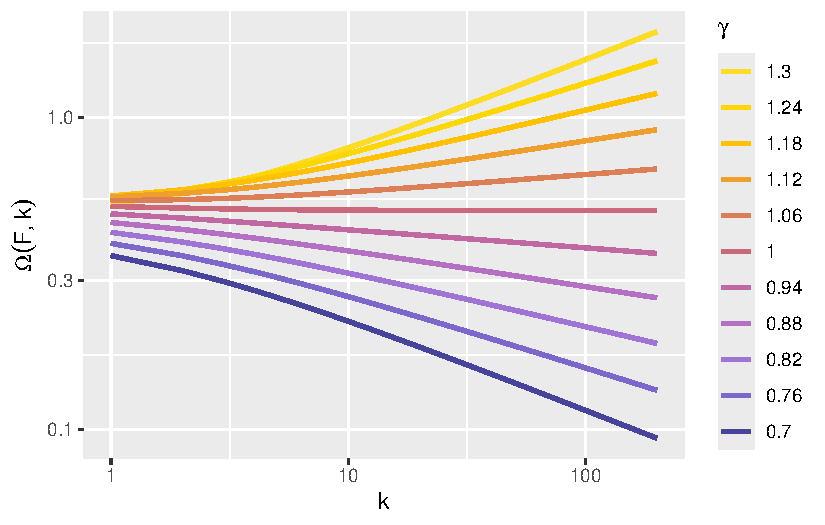
\includegraphics{doc_files/figure-pdf/fig-omega-1.pdf}

}

\caption{\label{fig-omega}Plot of \(\Omega(F,n)\) for various
\(\gamma \in (0.7,1.3)\)}

\end{figure}

Figure~\ref{fig-omega} shows that for \(\gamma<1\) \(\Omega(F,n)\) seems
to approach 0 as \(n\) increases, whereas for \(\gamma=1\)
\(\Omega(F,n)\) seems to converge to finite non-zero limit which is to
be expected as this corresponds to the BA model which has limiting
degree distribution in the Fréchet domain of attraction. However, for
\(\gamma>1\) the value of \(\Omega(F,n)\) appears to diverge and does
not approach a finite limit.

Shimura (2012) does not provide any results in particular for the case
of \(\Omega(F,n)\) diverging but if the definition of slow variation and
thus super-heavy tails is viewed as regular variation in the limit as
\(\alpha\) goes to infinity then the following can be obtained.

\begin{corollary}[]\protect\hypertarget{cor-omg}{}\label{cor-omg}

For a distribution \(F\) with survival function \(\overline F\) and some
\(n\in\mathbb Z^+\), if: \[
\lim_{n\rightarrow\infty} \Omega(F,n) = \lim_{\alpha\downarrow0} \alpha^{-1} = \infty
\] then \(F\) has super heavy tails

\end{corollary}

This is further supported by Figure~\ref{fig-shtail} below, which shows
the value of the quantity from Definition~\ref{def-sup} for increasing
values of \(n\) and values of \(\gamma\) in the range \((1,2)\). The
plot shows the quantity approaching \(1\) for all values of \(\gamma\)
as \(n\) increases, suggesting that the limiting degree distribution of
the GPA model with \(g(k) = k^\gamma,\gamma>1\) has super heavy tails.

\hypertarget{a-conjecture}{%
\section{A Conjecture}\label{a-conjecture}}

The results from this subsection suggest that for super-linear
preferential attachment functions the GPA model has limiting degree
distribution with super heavy tails. This, along with results for the
linear case in Section~\ref{sec-gen} and sub-linear cases in {[}NETSCI
BOOK{]} lead to the following conjecture.

\begin{conjecture}[]\protect\hypertarget{cnj-gpa}{}\label{cnj-gpa}

The GPA model is only capable of producing three different types of
degree distribution:

\begin{enumerate}
\def\labelenumi{\arabic{enumi}.}
\tightlist
\item
  Gumbel: sub-linear preferential attachment function
\item
  Fréchet \(\mathcal D(\Phi_2)\): linear preferential attachment
  function
\item
  Super heavy tails: super-linear preferential attachment function
\end{enumerate}

\end{conjecture}

This means that under the framework presented here, even the GPA model
is no where near close to being able to capture the range of types of
degree distribution found in real networks.

\begin{figure}[H]

{\centering 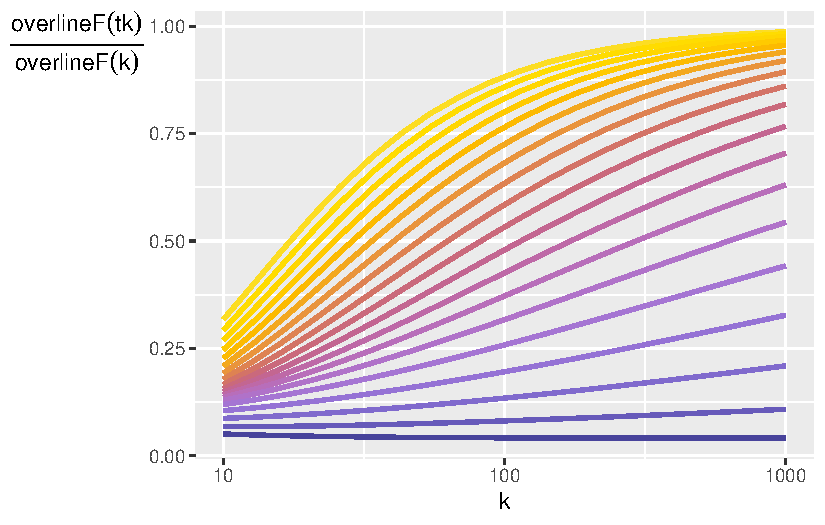
\includegraphics{doc_files/figure-pdf/fig-shtail-1.pdf}

}

\caption{\label{fig-shtail}Plot testing slow variation for
\(\gamma \in (1,2)\)}

\end{figure}

\hypertarget{next-steps}{%
\chapter{Next Steps}\label{next-steps}}

\appendix

\hypertarget{updated-project-plan}{%
\chapter{Updated Project Plan}\label{updated-project-plan}}

\hypertarget{training}{%
\chapter{Training}\label{training}}

\hypertarget{funding-and-stipend}{%
\section*{Funding and Stipend}\label{funding-and-stipend}}
\addcontentsline{toc}{section}{Funding and Stipend}

The funding for this project expires on \textbf{17th March 2027}.

\hypertarget{references}{%
\chapter*{References}\label{references}}
\addcontentsline{toc}{chapter}{References}

\hypertarget{refs}{}
\begin{CSLReferences}{1}{0}
\leavevmode\vadjust pre{\hypertarget{ref-agn22}{}}%
Ahmad, Touqeer, Carlo Gaetan, and Philippe Naveau. 2022. {``Modelling of
Discrete Extremes Through Extended Versions of Discrete Generalized
Pareto Distribution.''} \emph{ArXiv e-Prints}.
\url{https://arxiv.org/abs/2210.15253}.

\leavevmode\vadjust pre{\hypertarget{ref-Barabasi99}{}}%
Barabási, Albert-László, and Réka Albert. 1999. {``Emergence of Scaling
in Random Networks.''} \emph{Science} 286 (5439): 509--12.
\url{https://doi.org/10.1126/science.286.5439.509}.

\leavevmode\vadjust pre{\hypertarget{ref-fmh09}{}}%
Fraga Alves, Maria, Laurens Haan, and Cláudia Neves. 2009. {``A Test
Procedure for Detecting Super-Heavy Tails.''} \emph{Journal of
Statistical Planning and Inference} 139 (February).
\url{https://doi.org/10.1016/j.jspi.2008.04.026}.

\leavevmode\vadjust pre{\hypertarget{ref-hds24}{}}%
Hitz, Adrien S., Richard A. Davis, and Gennady Samorodnitsky. 2024.
{``Discrete Extremes.''} \emph{Journal of Data Science}, 1--13.
\url{https://doi.org/10.6339/24-JDS1120}.

\leavevmode\vadjust pre{\hypertarget{ref-shimura12}{}}%
Shimura, Takaaki. 2012. {``Discretization of Distributions in the
Maximum Domain of Attraction.''} \emph{Extremes} 15: 299--317.
\url{https://doi.org/10.1007/s10687-011-0137-7}.

\end{CSLReferences}



\end{document}
